\documentclass[12pt,a4paper]{article}

\usepackage{todonotes}

\newenvironment{mathprooftree}
  {\varwidth{.9\textwidth}\centering\leavevmode}
  {\DisplayProof\endvarwidth}
\usepackage{graphicx}
\graphicspath{{./imgs/}}
\usepackage{amsmath,amssymb,amsfonts,varwidth}
\usepackage{enumitem}
\usepackage{bussproofs}
\EnableBpAbbreviations{}
\usepackage{stackengine}
\usepackage{minted}
\usepackage{tikz}
\usetikzlibrary{arrows,shapes,automata,petri,positioning,calc,fit}
\tikzset{
    ASG/.style={
        circle,
        draw=black,
        minimum size=6mm,
    },
    lts/.style={
        circle,
        draw=black,
        fill=blue!6,
        minimum size=8mm,
   },
    prod/.style={
        ellipse,
        draw=black,
        fill=yellow!20,
        minimum size=8mm,
   },
    every edge/.style={
        draw,
        ->,>=stealth',
        auto,
        semithick
    },
    initial text = {},
    node distance=2.5cm,
    double distance=2pt,
  }
\tikzset{every loop/.style={min distance=7mm,in=120,out=60,looseness=2}}


% put your student ID here instead of 1234567

\newcommand{\thestudentid}{1803086}

% put the number of the question you are answering here, instead of 0

\newcommand{\theexam}{Programming Language Principals, Design and Implementation (Extended)}
\newcommand{\shorttheexam}{PLPDI (Extended)}

\author{ID \thestudentid}
\title{Exam for \theexam}
\date{}

\usepackage{cmbright}
\usepackage{fullpage}
\usepackage{fancyhdr}

\pagestyle{fancyplain}
\setlength{\headheight}{15pt}
\setlength{\headsep}{0.5cm}
\lhead{\fancyplain{ID \thestudentid}{ID \thestudentid}}
\rhead{\fancyplain{\theexam}{\theexam}}
\lfoot{\fancyplain{ID \thestudentid}{ID \thestudentid}}
\rfoot{\fancyplain{\shorttheexam}{\shorttheexam}}

\usepackage{hyperref}
\newcounter{question}\setcounter{question}{1}
\newenvironment{question}{%
\subsection*{Question \arabic{question}}}%
{\stepcounter{question}}

\begin{document}


\maketitle
After inserting your student ID and the module title in
the preamble, write your answers below.

\begin{question}

  \begin{enumerate}[label= (\alph*)]
    \item
          \[
            M = \lambda f: \mathbb{B} \rightarrow \mathbb{B}. \lambda g: \mathbb{B}\rightarrow \mathbb{B}. \lambda x: \mathbb{B}. \lambda y: \mathbb{B}. \texttt{if } x \texttt{ then } f y \texttt{ else } g y
          \]
          \begin{enumerate}[label= (\roman*)]
            \item
                  Prove $M$ is well typed

                  \begin{prooftree}

                    \AXC{}
                    \RL{\texttt{VAR} }
                    \UIC{$\Gamma \vdash x : \mathbb{B}$}


                    \AXC{}
                    \RL{\texttt{VAR} }
                    \UIC{$\Gamma \vdash f : \mathbb{B}\rightarrow \mathbb{B}$}

                    \AXC{}
                    \RL{\texttt{VAR} }
                    \UIC{$\Gamma \vdash y : \mathbb{B}$}

                    \RL{\texttt{APP} }
                    \BIC{$\Gamma \vdash fy : \mathbb{B}$}

                    \AXC{$\Pi_{1}$}

                    \RL{\texttt{ITE} }
                    \TIC{$\Gamma, y:\mathbb{B} \vdash \texttt{if } x \texttt{ then } f y \texttt{ else } g y: \mathbb{B}$}
                    \RL{\texttt{ABS} }
                    \UIC{$\Gamma, x:\mathbb{B} \vdash \lambda y: \mathbb{B}. \texttt{if } x \texttt{ then } f y \texttt{ else } g y: \mathbb{B}\rightarrow \mathbb{B}$}
                    \RL{\texttt{ABS} }
                    \UIC{$\Gamma,g:\mathbb{B}\rightarrow \mathbb{B} \vdash \lambda x: \mathbb{B}. \lambda y: \mathbb{B}. \texttt{if } x \texttt{ then } f y \texttt{ else } g y: \mathbb{B}\rightarrow \mathbb{B}\rightarrow \mathbb{B}$}
                    \RL{\texttt{ABS} }
                    \UIC{$f: \mathbb{B} \rightarrow \mathbb{B} \vdash  M_{1} :(\mathbb{B} \rightarrow \mathbb{B}) \rightarrow \mathbb{B} \rightarrow \mathbb{B} \rightarrow \mathbb{B} $}
                    \RL{\texttt{ABS}}
                    \UIC{$ \{  \} \vdash M : (\mathbb{B}\rightarrow \mathbb{B}) \rightarrow (\mathbb{B} \rightarrow \mathbb{B}) \rightarrow \mathbb{B} \rightarrow \mathbb{B} \rightarrow \mathbb{B}$}
                  \end{prooftree}

                  Where:

                  \begin{itemize}
                    \item $M_{1} = \lambda g: \mathbb{B}\rightarrow \mathbb{B}. \lambda x: \mathbb{B}. \lambda y: \mathbb{B}. \texttt{if } x \texttt{ then } f y \texttt{ else } g y$
                    \item $\Pi_{1}=$
                          \begin{prooftree}
                            \AXC{}
                            \RL{\texttt{VAR} }
                            \UIC{$\Gamma \vdash g: \mathbb{B}\rightarrow \mathbb{B}$}

                            \AXC{}
                            \RL{\texttt{VAR} }
                            \UIC{$\Gamma \vdash y:\mathbb{B}$}

                            \RL{\texttt{APP} }
                            \BIC{$\Gamma \vdash gy : \mathbb{B}$}
                          \end{prooftree}
                  \end{itemize}

            \item To produce the exclusive function from $M$ we can define the first order parameters $F$ and $G$ as follows:
                  \[
                    F = \lambda y:\mathbb{B}. \texttt{if } y \texttt{ then false}  \texttt{ else true}  : \mathbb{B}\rightarrow \mathbb{B}
                  \]
                  \[
                    G = \lambda y: \mathbb{B}. \texttt{if } y \texttt{ then true}  \texttt{ else false} : \mathbb{B}\rightarrow \mathbb{B}
                  \]
                  Alternatively, $G$ can simply be defined as the boolean identity function $\lambda y: \mathbb{B}. y : \mathbb{B}\rightarrow \mathbb{B}$. This is the definition I will use in latter parts of the question.

            \item
                  As the expression $(M F G \texttt{false } \texttt{true } )$ has type $\mathbb{B}$, we can be sure when using it that if we provide it to a function of type $\mathbb{B} \rightarrow T$ the evaluation will terminate and we will be returned a value of type $T$. Typed expressions do not get \textit{stuck}.

            \item

                  \begin{equation}
                    \begin{mathprooftree}
                      \AXC{}
                      \RL{$\beta$}
                      \UIC{$\lambda f: \mathbb{B}\rightarrow \mathbb{B}. M_{1} F \rightarrow_{v} \lambda g: \mathbb{B}\rightarrow \mathbb{B} \lambda x:\mathbb{B} \texttt{if } x \texttt{ then } Fy \texttt{ else } gy $}
                      \RL{$\texttt{CTX}_{(\bullet G)\texttt{false } \texttt{true } }$}
                      \UIC{\stackanchor{$(M F G) \texttt{false } \texttt{true }  \rightarrow_{v}$}{$((\lambda g: \mathbb{B}\rightarrow \mathbb{B} \lambda x:\mathbb{B} \texttt{if } x \texttt{ then } Fy \texttt{ else } gy )G) \texttt{false } \texttt{true }$}}
                    \end{mathprooftree}
                  \end{equation}

                  \begin{equation}
                    \begin{mathprooftree}
                      \AXC{}
                      \RL{$\beta$}
                      \UIC{\stackanchor{$(\lambda g: \mathbb{B}\rightarrow \mathbb{B}. \lambda x:\mathbb{B}. \texttt{if } x \texttt{ then } Fy \texttt{ else } gy )G \rightarrow_{v} $}{$\lambda x:\mathbb{B}.\lambda y:\mathbb{B}. \texttt{if } x \texttt{ then } Fy \texttt{ else } G y $}}
                      \RL{$\texttt{CTX} _{(\bullet) \texttt{false } \texttt{true } }$}
                      \UIC{\stackanchor{$((\lambda g: \mathbb{B}\rightarrow \mathbb{B}. \lambda x:\mathbb{B}. \texttt{if } x \texttt{ then } Fy \texttt{ else } gy )G) \texttt{false } \texttt{true } \rightarrow_{v} $}{$(\lambda x:\mathbb{B}.\lambda y:\mathbb{B}. \texttt{if } x \texttt{ then } Fy \texttt{ else } G y) \texttt{false } \texttt{true }  $}}
                    \end{mathprooftree}
                  \end{equation}

                  \begin{equation}
                    \begin{mathprooftree}
                      \AXC{}
                      \RL{$\beta$}
                      \UIC{\stackanchor{$(\lambda x:\mathbb{B}.\lambda y:\mathbb{B}. \texttt{if } x \texttt{ then } Fy \texttt{ else } G y) \texttt{false } \rightarrow_{v}$}{$\lambda y:\mathbb{B}. \texttt{if } \texttt{false}  \texttt{ then } F y \texttt{ else } G y $}}
                      \RL{$\texttt{CTX} _{\bullet \texttt{true } }$}
                      \UIC{\stackanchor{$(\lambda x:\mathbb{B}.\lambda y:\mathbb{B}. \texttt{if } x \texttt{ then } Fy \texttt{ else } G y) \texttt{false } \texttt{true } \rightarrow_{v}  $}{$(\lambda y:\mathbb{B}. \texttt{if } \texttt{false}  \texttt{ then } F y \texttt{ else } G y) \texttt{true }  $}}
                    \end{mathprooftree}
                  \end{equation}

                  \begin{equation}
                    \begin{mathprooftree}
                      \AXC{}
                      \RL{$\beta$}
                      \UIC{\stackanchor{$(\lambda y:\mathbb{B}. \texttt{if } \texttt{false}  \texttt{ then } F y \texttt{ else } G y) \texttt{true } \rightarrow_{v}$}{$\texttt{if } \texttt{false }  \texttt{ then } F \texttt{true }  \texttt{ else } G \texttt{true }    $}}
                    \end{mathprooftree}
                  \end{equation}

                  \begin{equation}
                    \begin{mathprooftree}
                      \AXC{}
                      \RL{\texttt{IteF} }
                      \UIC{$\texttt{if } \texttt{false }  \texttt{ then } F \texttt{true }  \texttt{ else } G \texttt{true }  \rightarrow_{v} G \texttt{true }   $}
                    \end{mathprooftree}
                  \end{equation}

                  \begin{equation}
                    \begin{mathprooftree}
                      \AXC{}
                      \RL{$\beta$}
                      \UIC{$(\lambda y:\mathbb{B}.y) \texttt{true } \rightarrow_{v} \texttt{true } $}
                    \end{mathprooftree}
                  \end{equation}
                  Where:
                  \begin{itemize}
                    \item $M_{1}$ is as defined the same as in a)i) .
                  \end{itemize}

                  $ \texttt{true } \in V$, $\therefore$ $(MFG) \texttt{false } \texttt{true } $ computes to a value.
          \end{enumerate}
    \item
        \[
        \texttt{Stack } = \forall \alpha.( \mathbb{N} \rightarrow \alpha \rightarrow \alpha ) \rightarrow \alpha \rightarrow \alpha
        \]
          \begin{enumerate}[label= (\roman*)]
            \item
                  \[
                  \lambda \alpha.\lambda f: \mathbb{N} \rightarrow \alpha \rightarrow \alpha .\lambda x:\alpha .f 0(f 0 (f 1 x))
                  \]
            \item
                  \[
                  \texttt{peek} = \lambda d:\mathbb{N} .\lambda s: \texttt{Stack} .s \{ \mathbb{N} \rightarrow \mathbb{N} \} G I d
                  \]
                  Where:
                  \begin{itemize}
                    \item $G = \lambda n: \mathbb{N} .\lambda g: \mathbb{N} \rightarrow \mathbb{N} . \lambda x: \mathbb{N}. g n$
                    \item $I = \lambda x: \mathbb{N} .x$
                  \end{itemize}

                  \begin{prooftree}

                    \AXC{$\Pi_{1}$}

                    \AXC{$\Pi_{2}$}

                    \RL{\texttt{APP} }
                    \BIC{$\Gamma \vdash s \{ \mathbb{N} \rightarrow \mathbb{N}  \} G : (\mathbb{N} \rightarrow \mathbb{N} ) \rightarrow (\mathbb{N} \rightarrow \mathbb{N} )$}

                    \AXC{}
                    \RL{\texttt{VAR} }
                    \UIC{$\Gamma, x : \mathbb{N} \vdash x : \mathbb{N} $}
                    \RL{\texttt{ABS} }
                    \UIC{$\Gamma \vdash I : \mathbb{N} \rightarrow \mathbb{N} $}

                    \RL{\texttt{APP} }
                    \BIC{$\Gamma \vdash ((s \{ \mathbb{N} \rightarrow  \mathbb{N} \}G )I) : \mathbb{N} \rightarrow \mathbb{N}$}

                    \AXC{}
                    \RL{\texttt{VAR} }
                    \UIC{$\Gamma \vdash d : \mathbb{N} $}

                    \RL{\texttt{APP} }
                    \BIC{$\Gamma,s:\texttt{Stack} \vdash ((s \{ \mathbb{N} \rightarrow \mathbb{N} \} G) I) d : \mathbb{N} \rightarrow \texttt{Stack} \rightarrow \mathbb{N} : \mathbb{N}  $}
                    \RL{\texttt{ABS} }
                    \UIC{$d:\mathbb{N} \vdash \lambda s: \texttt{Stack} .s \{ \mathbb{N} \rightarrow \mathbb{N} \} G I d : \mathbb{N} \rightarrow \texttt{Stack} \rightarrow \mathbb{N} : \texttt{Stack} \rightarrow \mathbb{N}  $}
                    \RL{\texttt{ABS} }
                    \UIC{$ \{  \} \vdash \lambda d: \mathbb{N} .\lambda s: \texttt{Stack} .s \{ \mathbb{N} \rightarrow \mathbb{N} \} G I d : \mathbb{N} \rightarrow \texttt{Stack} \rightarrow \mathbb{N}  $}
                  \end{prooftree}


                  Where:
                  \begin{itemize}
                    \item $\Pi_{1}=$
                          \begin{prooftree}
                            \AXC{}
                            \RL{\texttt{VAR} }
                            \UIC{$\Gamma \vdash s: \texttt{State} $}
                            \RL{\texttt{TAPP} }
                            \UIC{$\Gamma \vdash s \{ \mathbb{N} \rightarrow \mathbb{N}  \} : ( \mathbb{N} \rightarrow (\mathbb{N} \rightarrow \mathbb{N} ) \rightarrow (\mathbb{N} \rightarrow \mathbb{N} ) ) \rightarrow (\mathbb{N} \rightarrow \mathbb{N} ) \rightarrow (\mathbb{N} \rightarrow \mathbb{N} )$}
                          \end{prooftree}
                    \item $\Pi_{2}=$
                          \begin{prooftree}
                            \AXC{}
                            \RL{\texttt{VAR} }
                            \UIC{$\Gamma \vdash g : \mathbb{N} \rightarrow \mathbb{N} $}

                            \AXC{}
                            \RL{\texttt{VAR} }
                            \UIC{$\Gamma \vdash n : \mathbb{N} $}

                            \RL{\texttt{APP} }
                            \BIC{$\Gamma,x:\mathbb{N} \vdash gn : \mathbb{N} $}
                            \RL{\texttt{ABS} }
                            \UIC{$\Gamma, g: \mathbb{N} \rightarrow \mathbb{N} \vdash \lambda x: \mathbb{N}. gn : \mathbb{N} \rightarrow \mathbb{N} $}
                            \RL{\texttt{ABS} }
                            \UIC{$\Gamma, n : \mathbb{N} \vdash \lambda g: \mathbb{N} \rightarrow \mathbb{N} . \lambda x:\mathbb{N} . gn : (\mathbb{N} \rightarrow \mathbb{N} ) \rightarrow \mathbb{N} \rightarrow \mathbb{N} $}
                            \RL{\texttt{ABS} }
                            \UIC{$\Gamma \vdash G : \mathbb{N} \rightarrow (\mathbb{N} \rightarrow \mathbb{N} ) \rightarrow \mathbb{N} \rightarrow \mathbb{N} $}
                          \end{prooftree}
                  \end{itemize}
            \item
                  Prove:
                  \[
                  \texttt{peek } d s_{2} \rightarrow_{v}^{*} m
                  \]

                    \begin{prooftree}
                      \AXC{}
                      \RL{$\beta$}
                      \UIC{$(\lambda d:\mathbb{N} .\lambda s: \texttt{Stack} .s \{ \mathbb{N} \rightarrow \mathbb{N}  \} GId )d \rightarrow_{v} \lambda s: \texttt{Stack}.s \{ \mathbb{N} \rightarrow \mathbb{N}  \} GId $ }
                      \RL{$\texttt{CTX}_{\bullet s_{2}}$}
                      \UIC{$\texttt{peek } d s_{2} \rightarrow_{v} (\lambda s: \texttt{Stack}. s \{ \mathbb{N} \rightarrow \mathbb{N}  \} G I d )s_{2} $}
                    \end{prooftree}

                  \begin{prooftree}
                    \AXC{}
                    \RL{$\beta$}
                    \UIC{$(\lambda s: \texttt{Stack} .s \{ \mathbb{N} \rightarrow \mathbb{N}  \} GId)s_{2} \rightarrow_{v} s_{2} \{ \mathbb{N} \rightarrow \mathbb{N}  \} GId $}
                  \end{prooftree}

                  \begin{prooftree}
                    \AXC{}
                    \RL{$T_{\beta}$}
                    \UIC{\stackanchor{$\lambda \alpha . \lambda f: \mathbb{N} \rightarrow \alpha \rightarrow \alpha . \lambda x: \alpha . f n ( f m x ) \{ \mathbb{N} \rightarrow \mathbb{N}  \} \rightarrow_{v}  $}{$\lambda f: \mathbb{N} \rightarrow (\mathbb{N} \rightarrow \mathbb{N} )\rightarrow (\mathbb{N} \rightarrow \mathbb{N} ). \lambda x: (\mathbb{N} \rightarrow \mathbb{N} ). f n (f m x)$}}
                    \RL{$\texttt{CTX} _{(\bullet G)I)d}$}
                    \UIC{\stackanchor{$((s_{2} \{ \mathbb{N} \rightarrow \mathbb{N}  \} G)I)d \rightarrow_{v}$}{$ (((\lambda f: \mathbb{N} \rightarrow (\mathbb{N} \rightarrow \mathbb{N}) \rightarrow (\mathbb{N} \rightarrow \mathbb{N} ). \lambda x: \mathbb{N} \rightarrow \mathbb{N} . f n (f m x))G)I)d $}}
                  \end{prooftree}

                  \begin{prooftree}
                    \AXC{}
                    \RL{$\beta$}
                    \UIC{\stackanchor{$(\lambda f: \mathbb{N} \rightarrow (\mathbb{N} \rightarrow \mathbb{N} )\rightarrow (\mathbb{N} \rightarrow \mathbb{N} ). \lambda x: \mathbb{N} \rightarrow \mathbb{N}. f n ( f m x))G \rightarrow_{v} $}{$\lambda x:\mathbb{N} \rightarrow \mathbb{N} . Gn(Gmx)$}}
                    \RL{$\texttt{CTX} _{((\bullet)I)d}$}
                    \UIC{\stackanchor{$ (((\lambda f: \mathbb{N} \rightarrow (\mathbb{N} \rightarrow \mathbb{N}) \rightarrow (\mathbb{N} \rightarrow \mathbb{N} ). \lambda x: \mathbb{N} \rightarrow \mathbb{N} . f n (f m x))G)I)d \rightarrow_{v} $}{$((\lambda x: \mathbb{N} \rightarrow \mathbb{N}. Gn(Gmx))I)d$}}
                  \end{prooftree}

                  \begin{prooftree}
                    \AXC{}
                    \RL{$\beta$}
                    \UIC{$(\lambda x:\mathbb{N} \rightarrow \mathbb{N} . Gn(Gmx))I \rightarrow_{v} Gn(GmI)$}
                    \RL{$\texttt{CTX} _{(\bullet)d}$}
                    \UIC{$((\lambda x: \mathbb{N} \rightarrow \mathbb{N}. Gn(Gmx))I)d \rightarrow_{v} (Gn(GmI)d)$}
                  \end{prooftree}

                  \begin{prooftree}
                    \AXC{}
                    \RL{$\beta$}
                    \UIC{$(\lambda n: \mathbb{N} . \lambda g: \mathbb{N} \rightarrow \mathbb{N} . \lambda x: \mathbb{N} . gn)n \rightarrow_{v} \lambda g: \mathbb{N} \rightarrow \mathbb{N} .\lambda x: \mathbb{N} . gn$}
                    \RL{$\texttt{CTX} _{(\bullet(GmI))d}$}
                    \UIC{$(Gn(GmI)d) \rightarrow_{v} ((\lambda g: \mathbb{N} \rightarrow \mathbb{N} . \lambda x:\mathbb{N} .gn)(GmI))d$}
                  \end{prooftree}

                  \begin{prooftree}
                    \AXC{}
                    \RL{$\beta$}
                    \UIC{$(\lambda n: \mathbb{N} \lambda g: \mathbb{N} \rightarrow \mathbb{N} \lambda x: \mathbb{N} .gn)m \rightarrow_{v} \lambda g: \mathbb{N} \rightarrow \mathbb{N} . \lambda x: \mathbb{N} .gm$}
                    \RL{$\texttt{CTX}_{((\lambda g: \mathbb{N} \rightarrow \mathbb{N} .\lambda x:\mathbb{N} .gn)(\bullet I))d} $}
                    \UIC{\stackanchor{$((\lambda g: \mathbb{N} \rightarrow \mathbb{N} . \lambda x:\mathbb{N} . gn)(GmI))d \rightarrow_{v}  $}{$((\lambda g: \mathbb{N} \rightarrow \mathbb{N} . \lambda x:\mathbb{N} .gn)((\lambda g:\mathbb{N} \rightarrow \mathbb{N} .\lambda x:\mathbb{N} .gm)I))d$}}
                  \end{prooftree}

                  \begin{prooftree}
                    \AXC{}
                    \RL{$\beta$}
                    \UIC{$(\lambda g: \mathbb{N} \rightarrow \mathbb{N} .\lambda x:\mathbb{N} .gm)I \rightarrow_{v} \lambda x:\mathbb{N} . Im$}
                    \RL{$\texttt{CTX}_{((\lambda g: \mathbb{N} \rightarrow \mathbb{N} . \lambda x:\mathbb{N} .gn)(\bullet))d} $}
                    \UIC{\stackanchor{$((\lambda g: \mathbb{N} \rightarrow \mathbb{N} . \lambda x:\mathbb{N} .gn)((\lambda g:\mathbb{N} \rightarrow \mathbb{N} .\lambda x:\mathbb{N} .gm)I))d \rightarrow_{v} $}{$((\lambda g:\mathbb{N} \rightarrow \mathbb{N} . \lambda x:\mathbb{N} .gn)(\lambda x:\mathbb{N} .Im))d$}}
                  \end{prooftree}


                  \begin{prooftree}
                    \AXC{}
                    \RL{$\beta$}
                    \UIC{$(\lambda g: \mathbb{N} \rightarrow \mathbb{N} . \lambda x: \mathbb{N} . gn)(\lambda x: \mathbb{N} . Im) \rightarrow_{v}  \lambda x: \mathbb{N} . (\lambda x: \mathbb{N} Im)n$}
                    \RL{$\texttt{CTX} _{(\bullet)d}$}
                    \UIC{\stackanchor{$((\lambda g:\mathbb{N} \rightarrow \mathbb{N} . \lambda x:\mathbb{N} .gn)(\lambda x:\mathbb{N} .Im))d \rightarrow_{v} $}{$(\lambda x:\mathbb{N} .(\lambda x:\mathbb{N} .Im)n)d$}}
                  \end{prooftree}

                  \begin{prooftree}
                    \AXC{}
                    \RL{$\beta$}
                    \UIC{$(\lambda x:\mathbb{N} .(\lambda x:\mathbb{N} .Im)n)d \rightarrow_{v} (\lambda x:\mathbb{N}. Im)n$}
                  \end{prooftree}

                  \begin{prooftree}
                    \AXC{}
                    \RL{$\beta$}
                    \UIC{$(\lambda x:\mathbb{N}. Im)n \rightarrow_{v} Im$}
                  \end{prooftree}

                  \begin{prooftree}
                    \AXC{}
                    \RL{$\beta$}
                    \UIC{$Im \equiv (\lambda x: \mathbb{N}. x)m \rightarrow_{v} m$}
                  \end{prooftree}

            \item an abstract \textit{stack} datatype can be defined as follows:

                  \begin{align*}
                    \texttt{pack } &\langle \texttt{Stack} , \langle s_{0}, \langle \texttt{push} , \langle \texttt{peek}, \texttt{pop}   \rangle  \rangle  \rangle  \rangle \\
                                   &\texttt{ as }  \\ &\exists \texttt{stack}. \texttt{stack} \times ( \mathbb{N} \rightarrow \texttt{stack} \rightarrow \texttt{stack} \times \\
                                   &( \texttt{stack} \rightarrow \mathbb{N} \rightarrow \mathbb{N}  \times \texttt{stack} \rightarrow \texttt{stack}  )   )
                  \end{align*}

                  Where:

                  \begin{itemize}
                    \item $s_{0} = \lambda \alpha .\lambda f: \mathbb{N} \rightarrow \alpha \rightarrow \alpha . \lambda x: \alpha . x$
                    \item $\texttt{Stack } = \forall \alpha.( \mathbb{N} \rightarrow \alpha \rightarrow \alpha ) \rightarrow \alpha \rightarrow \alpha$
                          \item \texttt{push, peek} and \texttt{pop}   are defined the same as in the exam booklet, over the (concrete) \texttt{Stack} type.
                  \end{itemize}
          \end{enumerate}
  \end{enumerate}

\end{question}
\newpage
\begin{question}
\[
  Y = \lambda y. (\lambda f. t(\lambda z.ffz))(\lambda f.t(\lambda z.ffz))
\]
\begin{enumerate}[label= (\alph*)]
  \item
        The following ASG was generated using SPARTAN and the following code:
        \begin{minted}{text}
          LAMBDA(;t.APP(
   LAMBDA(; f.
     APP(t, LAMBDA(; z.
                    APP(APP(f,f),z))
        )
   ),
   LAMBDA(; f.
     APP(t, LAMBDA(; z.
                    APP(APP(f,f),z))
        )
   )
))
        \end{minted}

        \begin{center}
          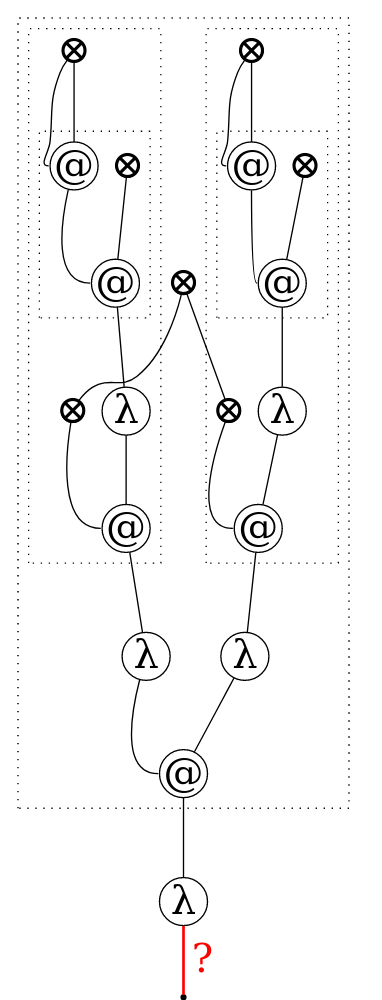
\includegraphics[scale=0.6]{YASG.png}
        \end{center}
  \item
        \begin{enumerate}[label= (\roman*)]
          \item
               \[
                Y(\lambda f.\lambda x.0)1
                \]

                \begin{center}
                  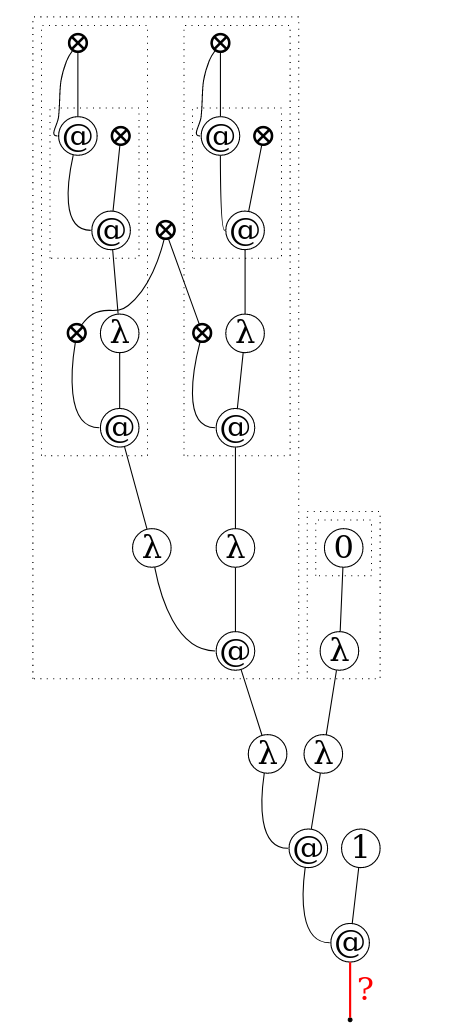
\includegraphics[scale=0.5]{2bi.png}
                \end{center}

                Firstly, the ASG evaluate the LHS, finding values on either side of the first application, it performs a reduction, replacing $\lambda t.$ with $\lambda f.\lambda x.0$:

                \begin{center}
                  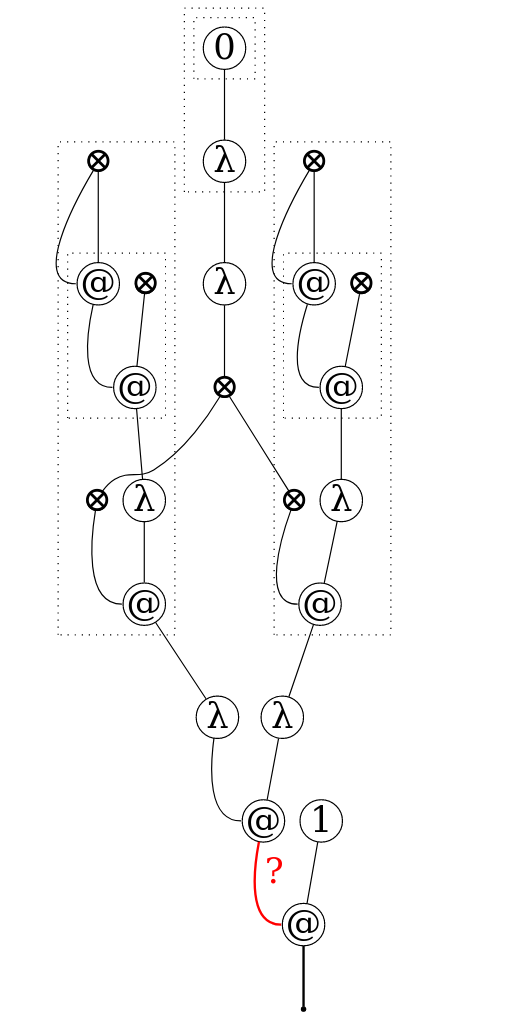
\includegraphics[scale=0.5]{2bi2.png}
                \end{center}

                It goes on to attempt to further evaluate the LHS, again finding two values either side of an application, the LH thunk is expanded attaching the RH value as its parameter:


                \begin{center}
                  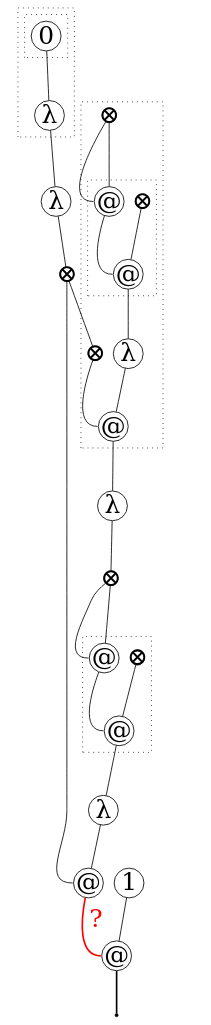
\includegraphics[scale=0.6]{2bi3.png}
                \end{center}

                Next, the machine performs a rewrite of a shared reference of $\lambda f.\lambda x.0$:

                \begin{center}
                  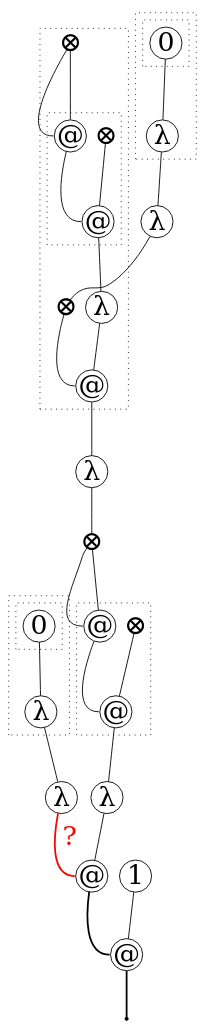
\includegraphics[scale=0.6]{2bi4.png}
                \end{center}

                Again finding two values on the LHS application, a reduction is performed, stripping the outer $\lambda $ from $\lambda f.\lambda x.0$, discarding the RHS.


                \begin{center}
                  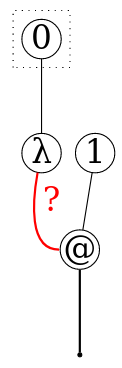
\includegraphics[scale=0.6]{2bi5.png}
                \end{center}

                Finally, finding 2 values either side of our application the system removes the next $\lambda $, leaving just $0$, our final result from this computation:


                \begin{center}
                  
\includegraphics[scale=0.6]{2bi6.png}
                \end{center}

          \item
                \[
                Y(\lambda f.\lambda x.f(x)*0)1
                \]

                This expression will diverge. This occurs as the second operand of the $*$ operator (1) is is never evaluated as our $Y$ combinator will infinitely expand over the first function argument $\lambda f.\lambda x.f(x)*0$

                After 91 steps of execution the ASG abstract machine will be in the following state:

                \begin{center}
                  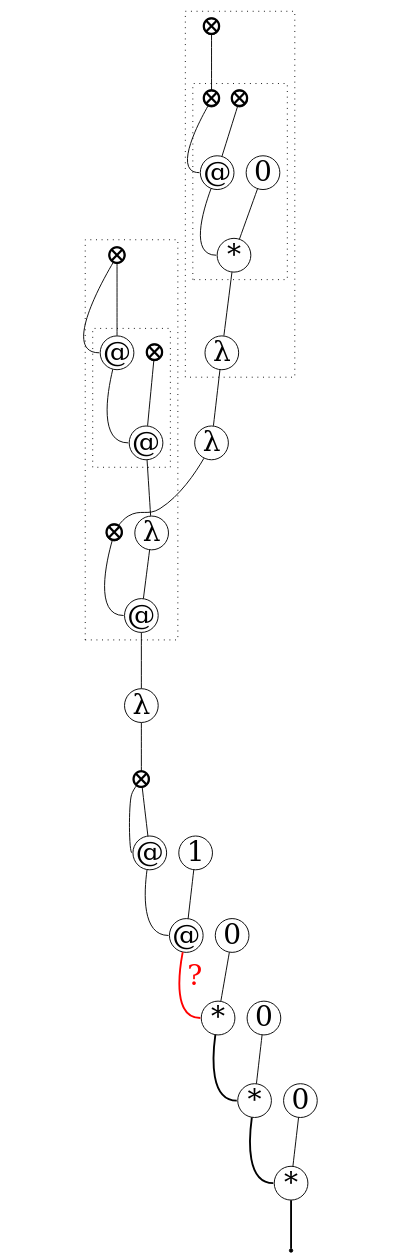
\includegraphics[scale=0.4]{2bii.png}
                \end{center}

                Intuitively, you can see that the second operand (1) is being pushed up as the $Y$ combinator duplicates the operation and first operand (0) infinitely.

          \item
                If we were to swap our operands to form an expression:

                \[
                Y(\lambda f.\lambda x.0*f(x))1
                \]

                This would terminate, due to the nature of our $*$ \textit{shortcut} operator which does not need to evaluate a second argument in the case where the first operand is 0.

                After 26 steps of execution we reach the following state:

                \begin{center}
                  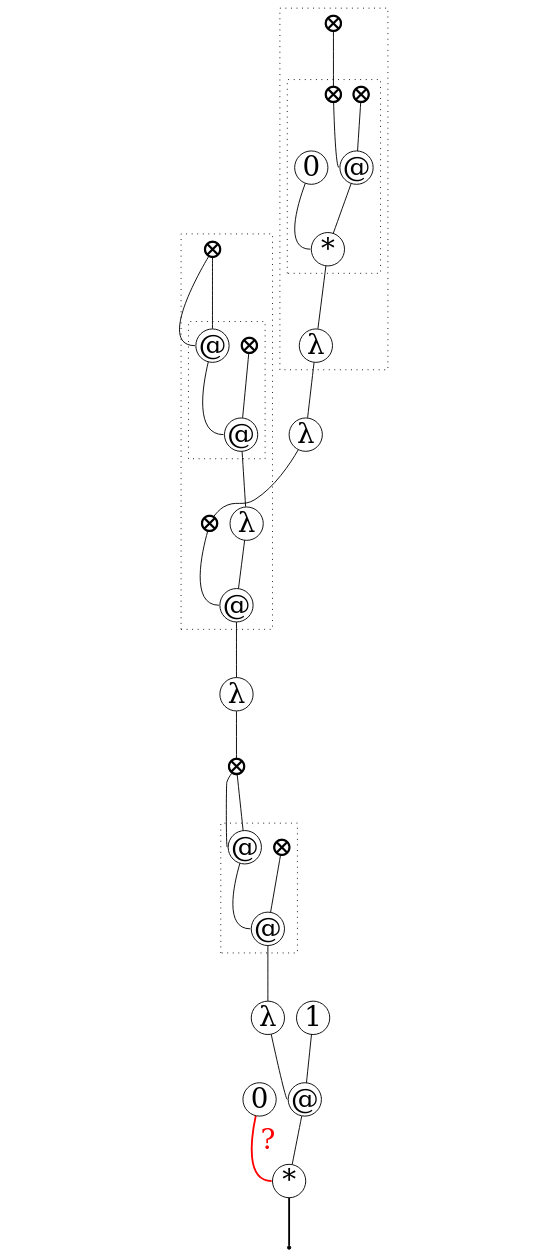
\includegraphics[scale=0.4]{2biii.png}
                \end{center}

                Here you can see that we have a state where we are attempting to evaluate $0*@$, with a traditional (eager) multiplication operator, we would find a value on the left and an expression on the right, forcing us to evaluate the RHS until we reach a value. However, our \textit{shortcut} operator allows us to instead skip this evaluate and return 0, eliminating the hang the Y combinator would otherwise cause. Our final result would be:

                \begin{center}
                  
\includegraphics[scale=0.6]{2bi6.png}
                \end{center}

        \end{enumerate}
  \item

        \begin{enumerate}[label =(\roman*)]
          \item
                My answer to b)i) would not be affected. Nor would my answer to b)ii) as the cause of the infinite expansion was the first argument, not the second.

                For b)iii) however, our answer would change. The program would no longer terminate as when it reached the state shown above, where $*$ is applied to a value (0) and an expression (@), it would be forced to expand the RHS application and create a similar infinite expansion as in b)ii) due to the use of the $Y$ combinator without a terminating condition.


          \item
                \textit{I feel like this is some sort of trick question, so I am going to explain my entire thought process}


                From a purely mathematical point of view, both $Y(\lambda f.\lambda x.f(x)*0)1$ and $Y(\lambda f.\lambda x.0*f(x))1$ can be optimised to $0$. However, I doubt any impure language would implement this optimisation. The possible side effects of executing $f(x)$ would be lost if it were removed. For instance, take the following code in Rust:

                \begin{minted}{rust}
                  fn f(_x:i32) -> i32{
                    println!("Some desired side effect");
                    2
                  }

                  fn main() {

                    let x = 2;
                    let res = 0*f(x);
                    println!("{}",res);

                  }
                \end{minted}

                Here we can see $f$ to have desirable side effects. The code produces the result $\texttt{Some desired side effect }$ followed by $0$, indicating that this optimisation is not made, keeping our desirable side effects.

                Our question however, is concerning the $\lambda$-Calculus, a mathematically pure language. Therefore, this optimisation would not lose any desirable side effects, as they are impossible, allowing us to optimise both expressions to $0$.


          \item
                Yes $Y(\lambda f.\lambda x.0)1$ can be optimised to $0$. This is the case as the result of evaluating the expression is not dependant on either of the parameters $f$ or $x$.
        \end{enumerate}

\end{enumerate}


\end{question}

\begin{question}
  \begin{enumerate}[label= (\alph*)]
    \item
          \begin{enumerate}[label= (\roman*)]
            \item
                  \textit{$a$ is true whenever $b$ is true.}

                  This is an example of an invariant, (a subset of \textit{safety properties}) as it can only be verified by checking $b \rightarrow a$ in each state individually. It can be represented in LTL as:
                  \[
                  \Box (b \rightarrow a)
                  \]

            \item
                  \textit{$a$ and $b$ are simultaneously true only a finite number of times.}

                  This is a \textit{liveness property} as only an infinite path could satisfy $\Box(a \wedge b)$ and given a path which violates it, we could easily extend it with a single state which satisfied $\neg (a \wedge b)$ to satisfy this property. In LTL it can be represented as:


                  \[
                  \Diamond \Box \neg (a \wedge b)
                  \]

            \item
                  \textit{every $b$ is immediately followed by an $a$}

                  This is an example of a \textit{safety property} as any trace violating this property would have a finite prefix in which a state satisfying $b$ is (immediately) followed by a state satisfying $\neg a$. Such a trace cannot be extended to satisfy the property. It can be written in LTL as


                  \[
                  \Box ( b \rightarrow \bigcirc a )
                  \]

            \item
                  \textit{exactly one of $a$ or $b$ (but not both) is eventually true.}

                  This is not a \textit{liveness property} as, given a trace violating this property by including a state in which $a$ and $b$ are true, we cannot add a suffix s.t. it no longer violates the property. Equally, it is not \textit{safety property} as an infinite path in which neither $a$ or $b$ is true does not satisfy the property and yet has no bad prefix.

                  \[
                  (\Diamond a \vee \Diamond b) \wedge (a \rightarrow \Box \neg b) \wedge (b \rightarrow \Box \neg a)
                  \]

            \item
                  \textit{if $a$ ever becomes true, then it remains true forever, and this is immediately preceded by a state where $b$ was true.}


                  This is a \textit{safety property}  as any violation would have a trace in which either the first occurrence of $a$ was not immediately preceded by a $b$ or the first occurrence of $a$ is eventually followed by a state in which $a$ is not true.

                  \[
                  ((b \wedge \bigcirc a ) \rightarrow \bigcirc \bigcirc \Box a) \vee \neg (\neg b \wedge \bigcirc a)
                  \]

          \end{enumerate}
    \item
          The first stage of LTL model checking is to negate the LTL formula $\Psi = \Box(b \rightarrow \bigcirc a)$:

          \begin{align*}
            \neg \Psi &= \neg\Box(b \rightarrow \bigcirc a) \\
                &= \Diamond \neg( b \rightarrow \bigcirc a ) \\
                &= \Diamond \neg (\neg b \vee \bigcirc a)\\
                &= \Diamond ( b \wedge \bigcirc \neg a )
          \end{align*}

          i.e. to prove that \textit{``every $b$ is immediately followed by an $a$''} does not hold, one must find a trace whereby a $b$ is immediately followed by $\neg a$.

          We then construct an NFA, $\mathcal{A}_{\Psi}$ of this formula:

          \begin{center}
            \begin{tikzpicture}
              \node [lts,initial] (q0) {$q_{0}$};
              \node [lts,right of=q0] (q1) {$q_{1}$};
              \node [lts,right of=q1,accepting] (q2) {$q_{2}$};

              \draw (q0) edge[loop above] node {$\neg b$ } (q0);
              \draw (q0) edge[->,bend left] node[above] {$b$} (q1);
              \draw (q1) edge[->,bend left] node[above] {$a \wedge \neg b$} (q0);
              \draw (q1) edge[->,loop above] node[above] {$b$} (q1);
              \draw (q1) edge node[above] {$\neg a$} (q2);
            \end{tikzpicture}
          \end{center}


          We then take the product of the LTS given in the question and the NFA $\mathcal{A}_{\Psi}$, defined above, to produce:

          $\mathcal{A}_{\Psi} \otimes M$, where $M$ is the LTS given in the question:


          \begin{center}
            
\begin{tikzpicture}
              \node [prod,initial] (s0q0) {$s_{0}q_{0}$};
              \node [prod, right of=s0q0] (s1q1) {$s_{1}q_{1}$};
              \node [prod, right of=s1q1] (s2q1) {$s_{2}q_{1}$};
              \node [prod,right of=s2q1, accepting, label=right:{$ \{ \texttt{accept}  \} $}] (s0q2) {$s_{0}q_{2}$};

              \draw (s0q0) edge (s1q1);
              \draw (s1q1) edge[bend left] (s2q1);
              \draw (s2q1) edge[bend left] (s1q1);
              \draw (s2q1) edge (s0q2);
            \end{tikzpicture}
          \end{center}

          Above you can see that the product of the NFA and LTS has an \textit{accept} state, meaning there exists a trace that satisfies the negation of the property, i.e. the property does not hold for all possible traces.

    \item
          The revised property can be expressed as:

          \[
            \Box (a \rightarrow \Diamond^{\leq k} b)
          \]

          A simple negation of this property, for checking, could be:

          \[
          \Diamond (a \wedge \neg \Diamond^{\leq k}b)
          \]


          In order to check this property over the LTS in the question, we would require a mechanism of \textit{counting} occurrences of non-$b$ states following an $a$.

          A simple implementation of this would be, for a fixed $k$, to add $k$ extra states to our NFA, where in each state ($1..k$) we could either continue waiting or return to the initial state. The final state could either find a $b$ and return to the initial state or terminate in an error state.

          An example for $k=2$ could be:


          \begin{center}
            \begin{tikzpicture}
              \node [lts,initial] (q0) {$q_{0}$};
              \node [lts,right of=q0] (q1) {$q_{1}$};
              \node [lts,right of=q1] (q2) {$q_{2}$};
              \node [lts,right of=q2,accepting] (q3) {$q_{3}$};

              \draw (q0) edge[loop above] node {$\neg a$ } (q0);
              \draw (q0) edge[->,bend left] node[above] {$a$} (q1);
              \draw (q1) edge[->,bend left] node[above] {$b$} (q0);
              \draw (q1) edge[->] node[above] {$\neg b$} (q2);
              \draw (q2) edge[bend left] node[below] {$b$} (q0);
              \draw (q2) edge[->] node[above] {$\neg b$} (q3);

            \end{tikzpicture}
          \end{center}

          The product of the above NFA and the given LTS would show whether the property could be violated.

          In a more general sense, the $\Diamond^{\leq k}\psi$ operator could be incorporated into LTL model checking by constructing it's negation as a series of $k$ linear states followed by a terminating state. In each of these $k$ states, if $\psi$ was true the NFA will return to the initial state and if $\psi$ was not true it would continue to the next state until it reached the final, accepting, position.

  \end{enumerate}
\end{question}

\newpage

\vspace*{1cm}
\pagebreak[3]\fbox{%
  \begin{minipage}[c]{0.92\textwidth}
    \raggedright{}
    Statement of good academic conduct

    By submitting this assignment, I understand that I am agreeing to the
    following statement of good academic conduct.
    \begin{itemize}
      \item
            I confirm that this assignment is my own work and I have not worked
            with others in preparing this assignment.
      \item
            I confirm this assignment was written by me and is in my own words,
            except for any materials from published or other sources which are
            clearly indicated and acknowledged as such by appropriate referencing.
      \item
            I confirm that this work is not copied from any other person's work
            (published or unpublished), web site, book or other source, and has
            not previously been submitted for assessment either at the University
            of Birmingham or elsewhere.
      \item
            I confirm that I have not asked, or paid, others to prepare any part
            of this work for me.
      \item
            I confirm that I have read and understood the
            \href{https://intranet.birmingham.ac.uk/as/registry/policy/conduct/plagiarism/index.aspx}{University
              regulations on plagiarism}.
    \end{itemize}

  \end{minipage}%
}
\end{document}

%%% Local Variables:
%%% mode: latex
%%% TeX-master: t
%%% End:
